\documentclass[11pt,a4paper]{article}

\usepackage[utf8]{inputenc}
\usepackage[T1]{fontenc}
\usepackage[spanish,es-tabla]{babel}
\usepackage[margin=2.5cm]{geometry}
\usepackage{graphicx}
\usepackage{booktabs}
\usepackage{tabularx}
\usepackage{float}
\usepackage{tikz}
\usepackage{circuitikz}
\usepackage{caption}
\usepackage{enumitem}
\usepackage[hidelinks]{hyperref}

\usetikzlibrary{shapes.geometric, arrows.meta, positioning, calc}

\graphicspath{{imagenes/}}
\captionsetup{font=small, labelfont=bf}
\renewcommand{\arraystretch}{1.15}

%------------------------------------------------------------------
\title{\vspace{-1.5cm}\textbf{Lista de Componentes}\\[0.3cm]
\large Manilla Inteligente de Seguridad para Mineros}
\author{Franco Parra \\ \small Internet de las Cosas --- Universidad Católica Boliviana}
\date{\today}

\begin{document}
\maketitle

%==================================================================
\section{Descripción del proyecto}

El proyecto consiste en desarrollar una \textbf{manilla inteligente para mineros}
que permita monitorear condiciones de seguridad del ambiente y del trabajador, y
comunicarse con una estación central mediante Wi-Fi.

La manilla utiliza una \textbf{Raspberry Pi Zero 2 W} como controlador principal.
Esta lee continuamente el sensor de monóxido de carbono \textbf{SEN0564} a
través de un conversor \textbf{ADS1115}, y la temperatura mediante el
termómetro infrarrojo \textbf{MLX90614}. Los valores y las advertencias se muestran en una pantalla
\textbf{OLED}, y tres botones permiten recorrer el menú. Ante una condición
peligrosa o un aviso de la central, la manilla avisa por tres canales
simultáneos: \textbf{vibración}, \textbf{sonido} (buzzer activo) y
\textbf{luz} (LED RGB). Los mensajes de voz se graban con el micrófono digital
\textbf{INMP441} y se envían, junto con lecturas y reportes, a la
\textbf{Raspberry Pi 4}, que actúa como servidor central de una o varias manillas.

\textbf{Alcance de la versión implementada:} el menú OLED y los tres botones
funcionan, y envían mensajes predeterminados de ayuda, estado y emergencia
mediante WebSocket, con cola local y confirmación de recepción. La central
incluye login, usuarios, asignaciones de manillas, mensajes en tiempo real y
lecturas recibidas. Los controladores de los sensores, el micrófono, el
buzzer, el LED RGB y el motor vibrador están definidos en este documento y en
la guía de conexiones, pero aún deben integrarse en el software.

\begin{figure}[H]
\centering
\resizebox{\textwidth}{!}{%
\begin{tikzpicture}[
  bloque/.style={draw, rounded corners, align=center, font=\small\sffamily,
                 minimum height=0.8cm, minimum width=2.5cm, fill=gray!8},
  nucleo/.style={bloque, fill=blue!12, thick, minimum height=1.3cm},
  flecha/.style={-{Latex[length=2.5mm]}, thick},
  etiqueta/.style={font=\scriptsize\sffamily, above=-1pt, sloped, pos=0.45}]

  \node[nucleo] (zero) at (0,0) {Raspberry Pi\\Zero 2 W};

  % Entradas
  \node[bloque] (co)    at (-8.4, 1.0) {SEN0564\\monóxido (CO)};
  \node[bloque] (ads)   at (-4.4, 1.0) {ADS1115\\ADC 16 bits};
  \node[bloque] (mlx)   at (-4.4,-0.6) {MLX90614\\temperatura IR};
  \node[bloque] (mic)   at (-4.4,-2.1) {INMP441\\micrófono};
  \node[bloque] (btn)   at (-4.4, 2.6) {3 botones};

  % Salidas
  \node[bloque] (oled)  at (4.6, 2.6) {OLED SSD1306\\128$\times$64};
  \node[bloque] (led)   at (4.6, 1.1) {Módulo\\LED RGB};
  \node[bloque] (buz)   at (4.6,-0.4) {Módulo buzzer\\activo};
  \node[bloque] (vib)   at (4.6,-1.9) {Micro motor\\vibrador};

  \node[nucleo] (pi4) at (0,-3.9) {Raspberry Pi 4\\(servidor central)};

  \draw[flecha] (co)    -- node[etiqueta] {A0} (ads);
  \draw[flecha] (ads)   -- node[etiqueta] {I\textsuperscript{2}C} (zero);
  \draw[flecha] (mlx)   -- node[etiqueta] {I\textsuperscript{2}C} (zero);
  \draw[flecha] (mic)   -- node[etiqueta] {I\textsuperscript{2}S} (zero);
  \draw[flecha] (btn)   -- node[etiqueta] {GPIO} (zero);
  \draw[flecha] (zero)  -- node[etiqueta] {I\textsuperscript{2}C} (oled);
  \draw[flecha] (zero)  -- node[etiqueta] {3 GPIO} (led);
  \draw[flecha] (zero)  -- node[etiqueta] {GPIO} (buz);
  \draw[flecha] (zero)  -- node[etiqueta] {GPIO + NPN} (vib);
  \draw[flecha, {Latex[length=2.5mm]}-{Latex[length=2.5mm]}] (zero) --
        node[font=\scriptsize\sffamily, right] {Wi-Fi} (pi4);
\end{tikzpicture}}
\caption{Arquitectura general del sistema.}
\end{figure}

%==================================================================
\section{Lista de componentes}

\begin{table}[H]
\centering
\small
\begin{tabularx}{\textwidth}{@{}c>{\raggedright\arraybackslash}p{4.1cm}X>{\raggedright\arraybackslash}p{2.9cm}@{}}
\toprule
\textbf{N.\textsuperscript{o}} & \textbf{Componente} & \textbf{Función en el proyecto} & \textbf{Interfaz} \\
\midrule
1  & Raspberry Pi 4                       & Servidor central                          & Wi-Fi / Ethernet \\
2  & Raspberry Pi Zero 2 W                & Controlador de la manilla                 & --- \\
3  & Pantalla OLED SSD1306                & Menús, lecturas y alertas                 & I\textsuperscript{2}C (\texttt{0x3C}) \\
4  & 3 botones pulsadores                 & Navegación por el menú                    & 3 GPIO \\
5  & Fermion SEN0564 (CO)                 & Monóxido de carbono                       & Analógica (ADS1115) \\
6  & Sensor IR MLX90614                   & Temperatura sin contacto                  & I\textsuperscript{2}C (\texttt{0x5A}) \\
7  & Conversor ADC ADS1115 16 bits        & Lectura del sensor de CO                  & I\textsuperscript{2}C (\texttt{0x48}) \\
8  & Micrófono INMP441 (MEMS, I\textsuperscript{2}S) & Grabación de mensajes de voz  & I\textsuperscript{2}S \\
9  & Módulo buzzer activo                 & Alarma sonora                             & 1 GPIO \\
10 & Módulo LED RGB                       & Indicador luminoso de estado              & 3 GPIO \\
11 & Micro motor vibrador                 & Alerta háptica                            & 1 GPIO + transistor \\
\bottomrule
\end{tabularx}
\caption{Resumen de los componentes del sistema.}
\end{table}

\subsection*{Componentes auxiliares necesarios}

Los módulos se conectan directamente, sin resistencias adicionales. Los
siguientes elementos solo se necesitan para el micro motor vibrador (si es un
motor suelto de dos cables), la cabecera de pines y la alimentación.

\begin{table}[H]
\centering
\small
\begin{tabularx}{\textwidth}{@{}>{\raggedright\arraybackslash}p{5.2cm}cX@{}}
\toprule
\textbf{Elemento} & \textbf{Cant.} & \textbf{Uso} \\
\midrule
Transistor NPN 2N2222A o S8050             & 1 & Etapa de potencia del motor vibrador. \\
Resistencia 1\,k$\Omega$                   & 1 & Base del transistor. \\
Resistencia 10\,k$\Omega$                  & 1 & Mantiene el motor apagado durante el arranque. \\
Diodo 1N4148 o 1N5819                      & 1 & Protección contra la tensión inversa del motor. \\
Condensador cerámico 100\,nF               & 1 & Filtro de ruido en bornes del motor. \\
Cabecera macho 2$\times$20                 & 1 & Si la Zero 2 W viene sin pines soldados. \\
Fuente 5\,V/2{,}5\,A o batería de 5\,V & 1 & Alimentación de la manilla (ver Sección~\ref{sec:energia}). \\
\bottomrule
\end{tabularx}
\caption{Componentes auxiliares.}
\label{tab:auxiliares}
\end{table}

%==================================================================
\section{Descripción de cada componente}

%------------------------------------------------------------------
\subsection{Raspberry Pi 4 --- Servidor central}

\begin{figure}[H]
\centering
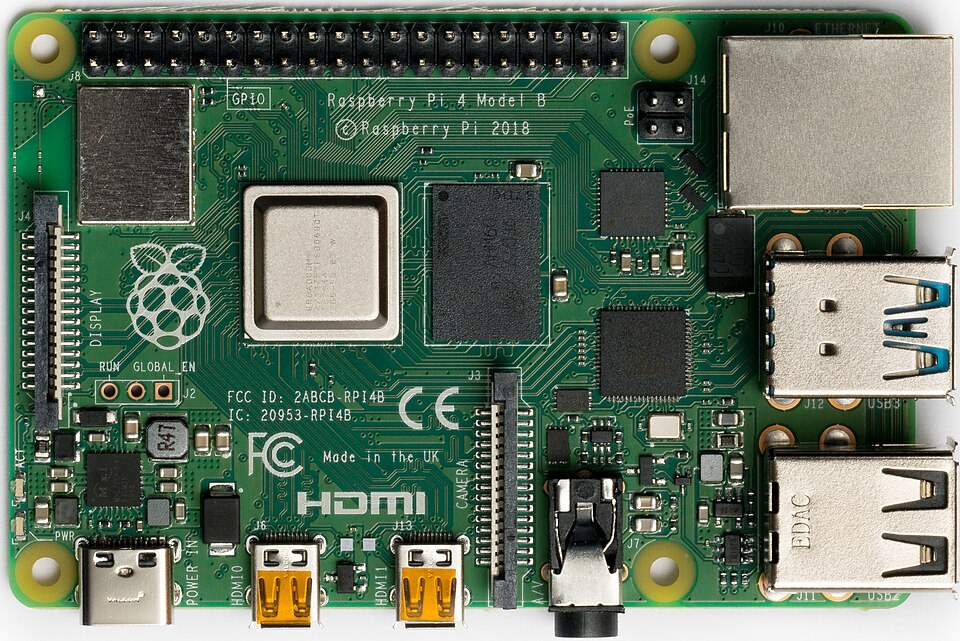
\includegraphics[width=0.42\textwidth]{rpi4.jpg}
\caption{Raspberry Pi 4 Modelo B.}
\end{figure}

Computador de placa única que funciona como \textbf{estación central}. Recibe por
red las lecturas, los reportes y los mensajes de voz de una o varias manillas, los
almacena y los muestra en la aplicación web.

\begin{itemize}[nosep]
  \item Procesador Broadcom BCM2711, cuatro núcleos Cortex-A72 a 1{,}5\,GHz.
  \item Memoria RAM de 2, 4 u 8\,GB (se recomienda 4\,GB).
  \item Wi-Fi 802.11ac de doble banda y Ethernet Gigabit.
  \item Alimentación de 5\,V/3\,A mediante USB-C.
\end{itemize}

\textbf{Uso previsto:} ejecutar con Docker la API ASP.NET Core, la base de datos
SQLite y la aplicación web React de la central. No se conecta por cables a la
manilla: ambas placas se comunican por la red.

%------------------------------------------------------------------
\subsection{Raspberry Pi Zero 2 W --- Cerebro de la manilla}

\begin{figure}[H]
\centering
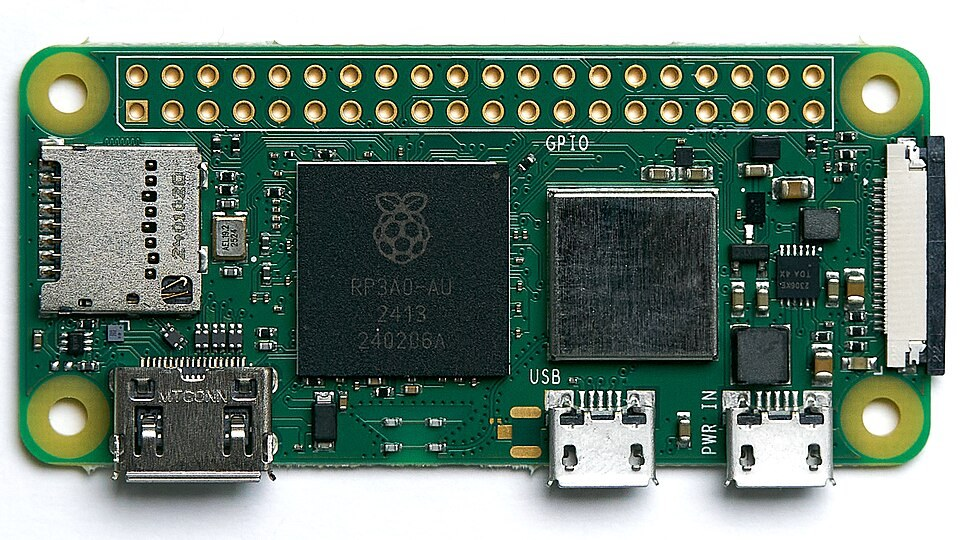
\includegraphics[width=0.42\textwidth]{rpizero2w.jpg}
\caption{Raspberry Pi Zero 2 W.}
\end{figure}

Controlador principal que se lleva en la muñeca. Se eligió por su tamaño reducido,
su bajo consumo y por incluir Wi-Fi, lo que evita añadir un módulo de
comunicación.

\begin{itemize}[nosep]
  \item Procesador de cuatro núcleos Cortex-A53 a 1\,GHz, 512\,MB de RAM.
  \item Wi-Fi 802.11 b/g/n de 2{,}4\,GHz y Bluetooth 4.2.
  \item 40 pines GPIO con buses I\textsuperscript{2}C, I\textsuperscript{2}S
        (PCM), SPI y UART.
  \item Dimensiones de 65 $\times$ 30\,mm.
  \item \textbf{No tiene entradas analógicas}: por eso se utiliza el ADS1115.
\end{itemize}

\textbf{Uso previsto:} leer los sensores y el micrófono, dibujar la interfaz en
la OLED, atender los botones, activar las alertas y enviar todo al servidor.

%------------------------------------------------------------------
\subsection{Pantalla OLED SSD1306 --- Interfaz visual}

\begin{figure}[H]
\centering
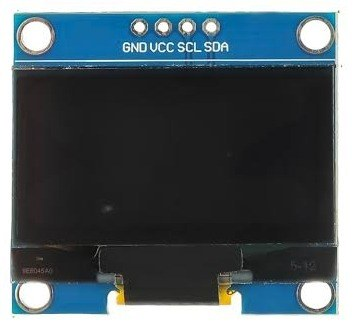
\includegraphics[width=0.36\textwidth]{oled.jpg}
\caption{Módulo de pantalla OLED de 0{,}96 pulgadas con controlador SSD1306.}
\end{figure}

Pantalla monocromática que muestra el menú, los valores de los sensores y las
advertencias. Al no necesitar retroiluminación consume poco y se lee bien en la
oscuridad de una mina.

\begin{itemize}[nosep]
  \item Resolución de 128 $\times$ 64 píxeles, tamaño de 0{,}96\,pulgadas.
  \item Comunicación por I\textsuperscript{2}C, dirección \texttt{0x3C}.
  \item Alimentación de 3{,}3\,V. Cuatro terminales: GND, VCC, SCL y SDA.
\end{itemize}

\textbf{Uso previsto:} menú de navegación (estado, gases, temperatura, mensajes y
ajustes) y pantallas de alerta. Es el componente que ya funciona con el
software actual.

%------------------------------------------------------------------
\subsection{Tres botones pulsadores --- Navegación}

\begin{figure}[H]
\centering
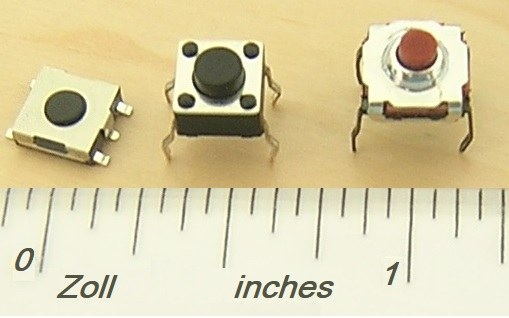
\includegraphics[width=0.34\textwidth]{botones.jpg}
\caption{Pulsadores táctiles del tipo utilizado en la manilla.}
\end{figure}

Tres pulsadores permiten manejar toda la interfaz sin pantalla táctil, lo que
resulta más práctico con guantes de trabajo.

\begin{itemize}[nosep]
  \item Botón 1 (GPIO 17): subir en el menú.
  \item Botón 2 (GPIO 27): bajar en el menú.
  \item Botón 3 (GPIO 22): seleccionar o confirmar.
\end{itemize}

\textbf{Conexión:} cada botón une su GPIO con GND al pulsarlo. El programa activa
la resistencia \emph{pull-up} interna y filtra los rebotes durante 80\,ms, por lo
que no se necesitan resistencias externas.

%------------------------------------------------------------------
\subsection{Fermion SEN0564 --- Monóxido de carbono}

\begin{figure}[H]
\centering
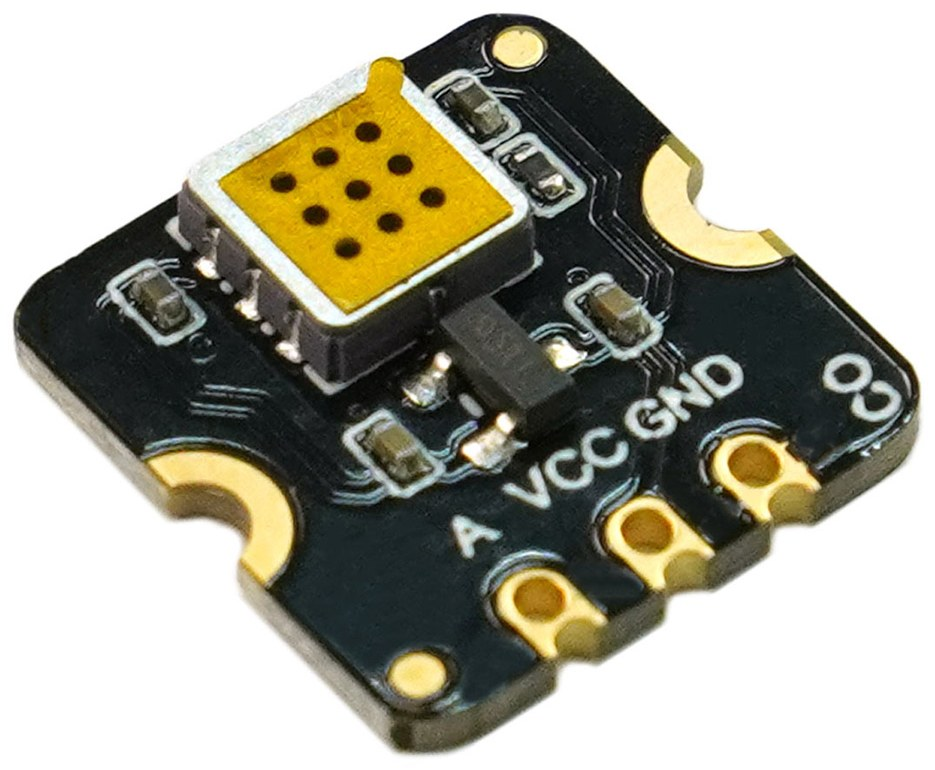
\includegraphics[width=0.36\textwidth]{sen0564.jpg}
\caption{DFRobot Fermion SEN0564, sensor MEMS de monóxido de carbono.}
\end{figure}

Sensor MEMS de monóxido de carbono (CO), uno de los gases más peligrosos en
minería: aparece tras las voladuras, en incendios y por la combustión de
equipos diésel. Es inodoro e incoloro, por lo que el minero no lo percibe.

\begin{itemize}[nosep]
  \item Rango de detección de 5 a 5000\,ppm de CO.
  \item Alimentación de 3{,}3 a 5\,V, consumo menor a 20\,mA.
  \item Salida analógica (terminales A, VCC y GND); la tensión de salida no
        supera la de alimentación.
  \item Tamaño de 13 $\times$ 13\,mm y bajo consumo, adecuado para un
        dispositivo portátil.
\end{itemize}

\textbf{Conexión:} alimentado a 3{,}3\,V, su salida va directamente a la entrada
A0 del ADS1115, sin resistencias adicionales. \textbf{Importante:} el fabricante indica
que es un sensor \emph{cualitativo}; para expresar el resultado en ppm se
requiere calibración.

%------------------------------------------------------------------
\subsection{Sensor infrarrojo de temperatura MLX90614}

\begin{figure}[H]
\centering
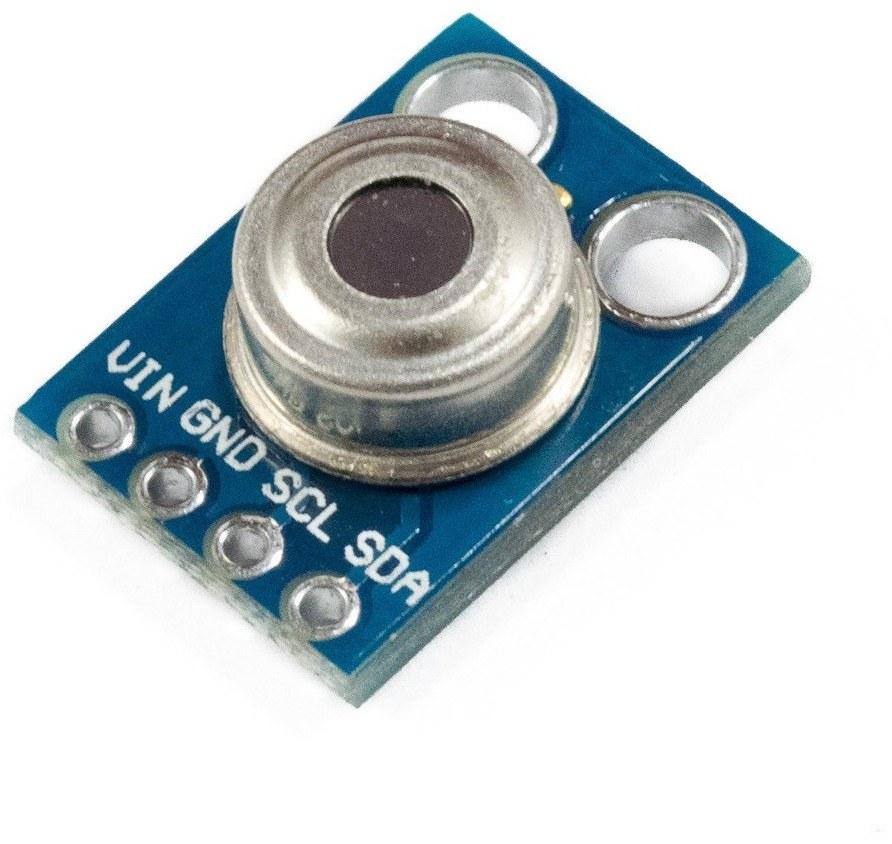
\includegraphics[width=0.34\textwidth]{mlx90614.jpg}
\caption{Módulo de termómetro infrarrojo sin contacto MLX90614 (GY-906).}
\end{figure}

Mide la temperatura a distancia captando la radiación infrarroja de un cuerpo u
objeto. Entrega además la temperatura ambiente del propio sensor.

\begin{itemize}[nosep]
  \item Rango de $-40$ a $+125\,^{\circ}$C en ambiente y de $-70$ a
        $+380\,^{\circ}$C en objeto.
  \item Precisión aproximada de $\pm 0{,}5\,^{\circ}$C cerca de la temperatura
        ambiente.
  \item Comunicación I\textsuperscript{2}C (SMBus), dirección \texttt{0x5A}.
  \item Alimentación de 3{,}3\,V (existen variantes de 5\,V).
\end{itemize}

\textbf{Uso previsto:} vigilar la temperatura del túnel y detectar focos de calor
anómalos. Comparte el bus I\textsuperscript{2}C con la OLED y el ADS1115.
\textbf{Montaje:} dejar su ventana despejada y orientada hacia el exterior de la
carcasa.

%------------------------------------------------------------------
\subsection{Conversor ADC ADS1115}
\label{sec:adc}

\begin{figure}[H]
\centering
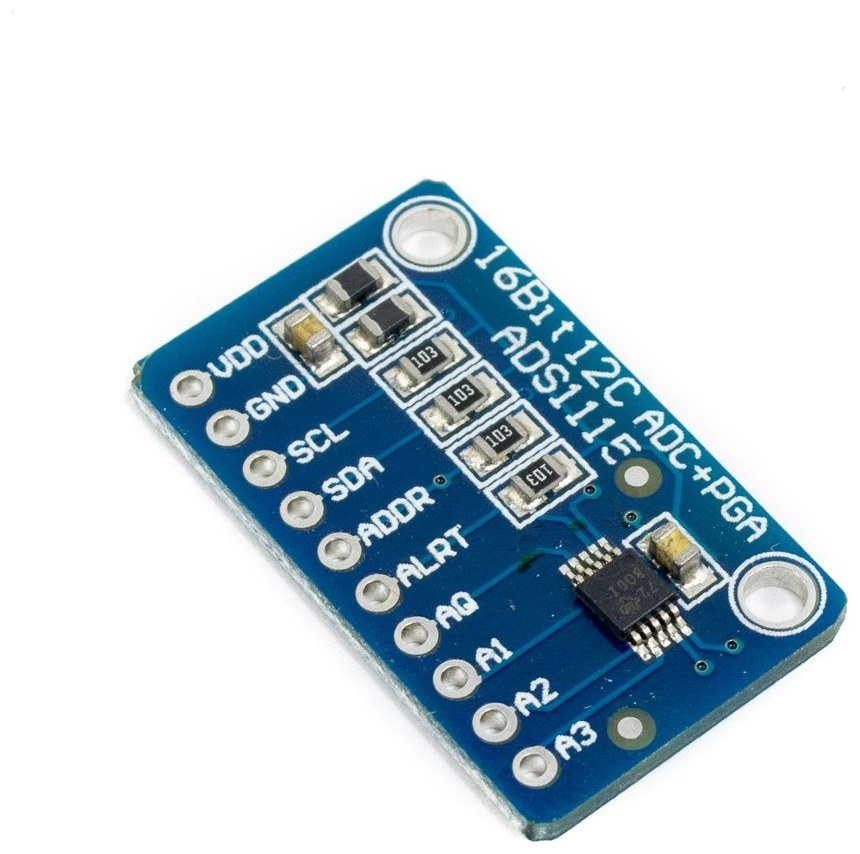
\includegraphics[width=0.34\textwidth]{ads1115.jpg}
\caption{Módulo conversor analógico-digital ADS1115.}
\end{figure}

La Raspberry Pi Zero 2 W \emph{no posee entradas analógicas}, mientras que el
SEN0564 entrega una señal analógica. El ADS1115 la convierte a un valor digital
y lo envía por I\textsuperscript{2}C.

\begin{itemize}[nosep]
  \item Resolución de 16 bits y amplificador de ganancia programable.
  \item Cuatro entradas simples: A0 (SEN0564); A1, A2 y A3 quedan libres para
        futuros sensores.
  \item Comunicación I\textsuperscript{2}C, dirección \texttt{0x48} con ADDR a GND.
  \item Alimentación de 3{,}3\,V para mantener el bus a la tensión de la Pi.
  \item Hasta 860 muestras por segundo, más que suficiente para un sensor de gas.
\end{itemize}

\textbf{Límite de entrada:} alimentado a 3{,}3\,V, ninguna entrada debe superar
3{,}6\,V. El SEN0564 alimentado a 3{,}3\,V cumple este límite sin adaptación.

%------------------------------------------------------------------
\subsection{Micrófono digital INMP441 (MEMS, I\textsuperscript{2}S)}

\begin{figure}[H]
\centering
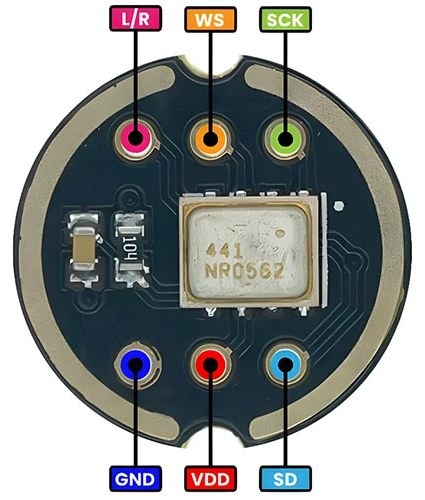
\includegraphics[width=0.30\textwidth]{inmp441.jpg}
\caption{Módulo de micrófono INMP441 y sus terminales.}
\end{figure}

Micrófono MEMS omnidireccional con conversor analógico-digital integrado. Entrega
el audio ya digitalizado por el bus I\textsuperscript{2}S, que la Raspberry Pi
lee directamente.

\begin{itemize}[nosep]
  \item Salida digital I\textsuperscript{2}S de 24 bits.
  \item Respuesta de 60\,Hz a 15\,kHz y relación señal/ruido de 61\,dBA.
  \item Alimentación de 1{,}8 a 3{,}3\,V, consumo de 1{,}4\,mA.
        \textbf{No admite 5\,V.}
  \item Terminales: SCK, WS, SD, L/R, VDD y GND.
\end{itemize}

\textbf{Uso previsto:} grabar mensajes de voz cortos, guardarlos localmente y
enviarlos a la Raspberry Pi 4. \textbf{Ventaja frente al diseño anterior:} el
micrófono analógico MAX9814 dependía del ADS1115, cuyo máximo de 860
muestras/s es insuficiente para voz. El INMP441 graba a 48\,kHz sin usar el
ADC.

%------------------------------------------------------------------
\subsection{Módulo buzzer activo --- Alarma sonora}

\begin{figure}[H]
\centering
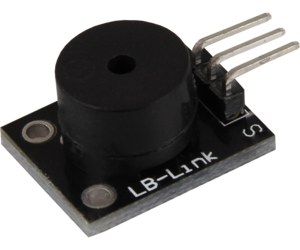
\includegraphics[width=0.26\textwidth]{buzzer.jpg}
\caption{Módulo de buzzer activo (referencia KY-012).}
\end{figure}

Zumbador con oscilador interno: suena con solo recibir un nivel lógico, sin
necesidad de generar una señal PWM.

\begin{itemize}[nosep]
  \item Tono fijo de aproximadamente 2{,}5\,kHz.
  \item Alimentación de 3{,}3 a 5\,V; consumo de 20 a 30\,mA.
  \item Se controla desde un único pin GPIO (GPIO 24).
  \item Según el modelo se activa con nivel alto o con nivel bajo.
\end{itemize}

\textbf{Uso previsto:} alarma audible ante gas o temperatura peligrosos.
\textbf{Importante:} alimentarlo a 3{,}3\,V. Los módulos con transistor PNP
alimentados a 5\,V no se apagan con los 3{,}3\,V de la Pi y pueden devolver
tensión al GPIO.

%------------------------------------------------------------------
\subsection{Módulo LED RGB --- Indicador de estado}

\begin{figure}[H]
\centering
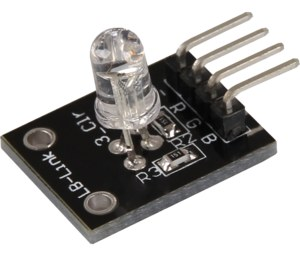
\includegraphics[width=0.26\textwidth]{led-rgb.jpg}
\caption{Módulo LED RGB de cátodo común (referencia KY-016).}
\end{figure}

LED con tres emisores (rojo, verde y azul) en una misma cápsula. Combinándolos
se obtienen distintos colores para indicar el estado de la manilla de un
vistazo.

\begin{itemize}[nosep]
  \item Terminales R, G, B y común (\textbf{--} en cátodo común, \textbf{+} o
        \textbf{V} en ánodo común).
  \item Un GPIO por color: GPIO 5 (R), GPIO 6 (G) y GPIO 13 (B).
  \item Brillo regulable con PWM por software.
\end{itemize}

\textbf{Uso propuesto:} verde para funcionamiento normal, amarillo para
precaución, rojo para peligro y azul para mensajes o falta de conexión.
\textbf{Importante:} si la placa no incluye resistencias limitadoras, añadir
una en serie con cada color (ver la guía de conexiones).

%------------------------------------------------------------------
\subsection{Micro motor vibrador --- Alerta háptica}

\begin{figure}[H]
\centering
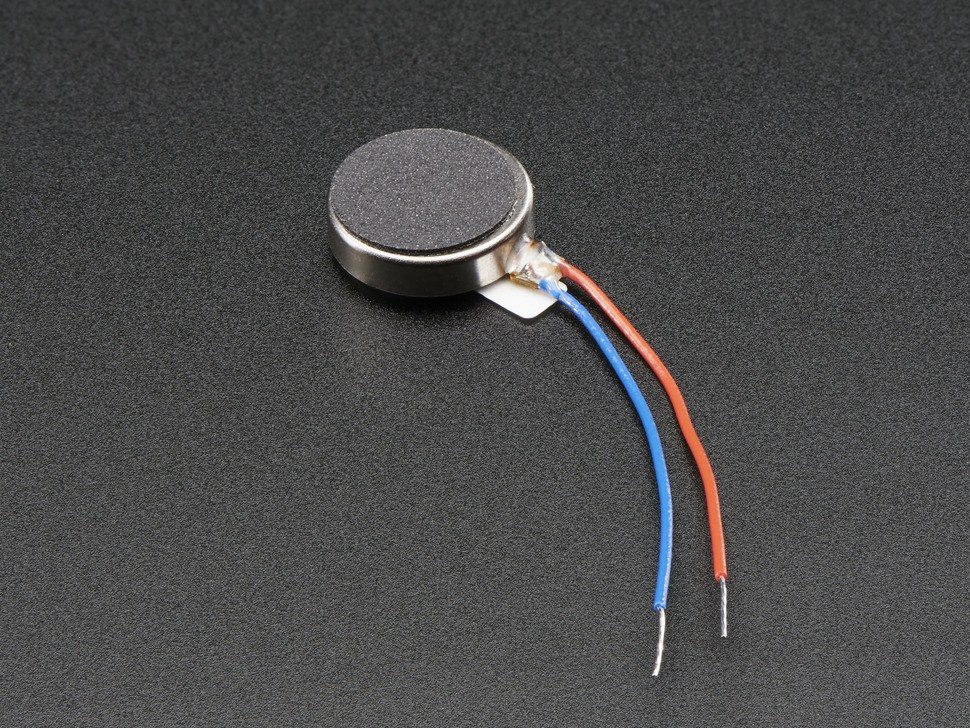
\includegraphics[width=0.34\textwidth]{motor-vibrador.jpg}
\caption{Micro motor vibrador de tipo moneda (10\,mm).}
\end{figure}

Motor con masa excéntrica que genera vibración. Es el canal de aviso más fiable
en una mina, donde el ruido puede impedir oír la alarma y la vista puede estar
ocupada.

\begin{itemize}[nosep]
  \item Tensión nominal típica de 3\,V (rango de 2 a 5\,V según el modelo).
  \item Consumo de 60 a 80\,mA a 3\,V, con un pico mayor al arrancar.
  \item Dos cables: positivo (rojo) y negativo (azul o negro).
\end{itemize}

\textbf{Importante:} un GPIO solo entrega unos pocos miliamperios, por lo que el
motor \textbf{no se conecta directamente al GPIO}. Se maneja con un transistor
NPN, una resistencia de base y un diodo de protección. \textbf{Uso previsto:}
vibración larga ante peligro, vibración doble al recibir un aviso y vibración
corta como confirmación al pulsar un botón.

%==================================================================
\section{Resumen de conexiones}

\begin{table}[H]
\centering
\small
\begin{tabularx}{\textwidth}{@{}>{\raggedright\arraybackslash}p{3.6cm}X>{\raggedright\arraybackslash}p{1.9cm}@{}}
\toprule
\textbf{Componente} & \textbf{Bus / pines de la Zero 2 W} & \textbf{Alimentación} \\
\midrule
OLED SSD1306        & I\textsuperscript{2}C: SDA pin 3, SCL pin 5 --- \texttt{0x3C} & 3{,}3\,V \\
ADS1115             & I\textsuperscript{2}C: SDA pin 3, SCL pin 5 --- \texttt{0x48} & 3{,}3\,V \\
MLX90614            & I\textsuperscript{2}C: SDA pin 3, SCL pin 5 --- \texttt{0x5A} & 3{,}3\,V \\
SEN0564 (CO)        & A $\rightarrow$ ADS1115 A0 (directo)                             & 3{,}3\,V \\
INMP441             & I\textsuperscript{2}S: SCK GPIO 18 (pin 12), WS GPIO 19 (pin 35), SD GPIO 20 (pin 38); L/R a GND & 3{,}3\,V \\
Botones 1 / 2 / 3   & GPIO 17 (pin 11), GPIO 27 (pin 13), GPIO 22 (pin 15) a GND       & --- \\
Motor vibrador      & GPIO 23 (pin 16) $\rightarrow$ transistor NPN                    & 3{,}3\,V \\
Buzzer activo       & GPIO 24 (pin 18)                                                 & 3{,}3\,V \\
LED RGB             & R GPIO 5 (pin 29), G GPIO 6 (pin 31), B GPIO 13 (pin 33)         & --- \\
\bottomrule
\end{tabularx}
\caption{Interfaz eléctrica de cada componente con la Raspberry Pi Zero 2 W.}
\end{table}

Los tres dispositivos I\textsuperscript{2}C comparten el mismo par de líneas SDA y
SCL, ya que cada uno tiene una dirección distinta. El micrófono usa el bus
I\textsuperscript{2}S, independiente del anterior. Todos los módulos se alimentan
a 3{,}3\,V. La Figura~\ref{fig:cableado} muestra el diagrama de cableado completo.
El detalle de cada cable, la etapa del motor y las pruebas de montaje se
encuentran en el documento \texttt{conexiones.tex}.

\begin{figure}[p]
\centering
\resizebox{\textwidth}{!}{% Diagrama de cableado de la manilla. Fuente única para conexiones.tex y docs/imagenes/cableado.{png,svg}.
% Requiere: circuitikz y la biblioteca calc de TikZ.
% Tamaños de letra fijos: el diagrama se ve igual en documentos de 10 u 11 pt.
\def\cabS{\fontsize{7}{8.5}\selectfont}
\def\cabT{\fontsize{5}{6}\selectfont}
\begin{tikzpicture}[american, x=1cm, y=1cm, font=\sffamily\cabS,
  line cap=round, line join=round]
  \colorlet{c33}{orange!85!black}
  \colorlet{cSDA}{blue!75!black}
  \colorlet{cSCL}{cyan!65!black}
  \colorlet{cI2S}{violet!85!black}
  \colorlet{cBtn}{green!50!black}
  \colorlet{cOut}{teal!85!black}
  \colorlet{cAna}{brown!75!black}
  \colorlet{pcbBlue}{blue!50!black}
  \colorlet{pcbBlack}{black!85}
  \tikzset{
    wire/.style={line width=1.1pt},
    pcb/.style={draw=black!70, rounded corners=2pt, line width=0.6pt},
    pad/.style={circle, draw=black!60, fill=yellow!75!orange, inner sep=0pt, minimum size=4.5pt},
    hdr/.style={circle, draw=black!80, inner sep=0pt, minimum size=0.38cm, font=\sffamily\cabT\bfseries},
    union/.style={circle, fill, inner sep=0pt, minimum size=4.5pt},
    piname/.style={font=\sffamily\cabT, text=white},
    title/.style={font=\sffamily\cabS\bfseries, text=white},
    etq/.style={font=\sffamily\cabT, above=-1pt},
    vcc/.pic={\draw[c33, line width=1.1pt] (0,0) -- (0,-0.3);
              \draw[c33, line width=1.8pt] (-0.15,-0.3) -- (0.15,-0.3);
              \node[c33, font=\sffamily\cabT\bfseries, below=-1pt] at (0,-0.32) {3,3V};},
    vccup/.pic={\draw[c33, line width=1.1pt] (0,0) -- (0,0.3);
                \draw[c33, line width=1.8pt] (-0.15,0.3) -- (0.15,0.3);
                \node[c33, font=\sffamily\cabT\bfseries, above=-1pt] at (0,0.32) {3,3V};},
    tierra/.pic={\draw[line width=1.1pt] (0,0) -- (0,-0.22) node[ground, scale=0.75]{};},
  }

  %================ Cabecera GPIO de la Raspberry Pi Zero 2 W
  \fill[green!35!black, rounded corners=3pt] (-0.75,0.45) rectangle (0.75,-11.85);
  \node[align=center, font=\sffamily\cabS\bfseries] at (1.2,1.15)
       {Raspberry Pi Zero 2 W\\[-1pt]{\normalfont\sffamily\cabT cabecera GPIO, pin 1 arriba a la izquierda}};
  \foreach \n/\c/\t in {
     1/c33/white,      2/red!55/black,    3/cSDA/white,      4/red!55/black,
     5/cSCL/white,     6/black/white,     7/white/black!50,  8/white/black!50,
     9/black!45/white, 10/white/black!50, 11/cBtn/white,     12/cI2S/white,
    13/cBtn/white,    14/black!45/white, 15/cBtn/white,     16/cOut/white,
    17/orange!35/black!60, 18/cOut/white, 19/white/black!50, 20/black!45/white,
    21/white/black!50, 22/white/black!50, 23/white/black!50, 24/white/black!50,
    25/black!45/white, 26/white/black!50, 27/black!20/black!50, 28/black!20/black!50,
    29/red!80!black/white, 30/black!45/white, 31/green!60!black/white, 32/white/black!50,
    33/blue!80/white, 34/black!45/white, 35/cI2S/white,     36/black!20/black!50,
    37/white/black!50, 38/cI2S/white,    39/black!45/white, 40/black!20/black!50} {
    \pgfmathsetmacro{\px}{isodd(\n) ? -0.35 : 0.35}
    \pgfmathsetmacro{\py}{-floor((\n-1)/2)*0.6}
    \node[hdr, fill=\c, text=\t] (p\n) at (\px,\py) {\n};
  }
  \node[right=3pt, text=black!55, font=\sffamily\cabT] at (p2.east) {5 V: no conectar};
  \node[right=3pt, text=black!55, font=\sffamily\cabT] at (p4.east) {5 V: no conectar};

  % Alimentación de las líneas de la protoboard
  \draw[wire, c33] (p1.west) -- (-0.95,0);
  \pic at (-0.95,0) {vccup};
  \draw[wire] (p6.east) -- (1.0,-1.2);
  \pic at (1.0,-1.2) {tierra};

  %================ Módulos I2C y sensor de CO (arriba)
  % OLED SSD1306
  \draw[pcb, fill=pcbBlue] (-7.45,4.0) rectangle (-5.2,5.75);
  \fill[black] (-7.2,4.75) rectangle (-5.45,5.45);
  \node[title] at (-6.325,5.1) {OLED SSD1306};
  \foreach \x/\l in {-7.0/GND, -6.55/VCC, -6.1/SCL, -5.65/SDA} {
    \node[pad] at (\x,4.0) {};
    \node[piname, above=2pt] at (\x,4.0) {\l};
  }
  % ADS1115
  \draw[pcb, fill=pcbBlue] (-4.95,4.0) rectangle (0.25,5.75);
  \node[title] at (-2.35,5.4) {ADS1115 (conversor ADC)};
  \foreach \x/\l in {-4.6/VDD, -4.1/GND, -3.6/SCL, -3.1/SDA, -2.6/ADDR,
                     -2.1/ALRT, -1.6/A0, -1.1/A1, -0.6/A2, -0.1/A3} {
    \node[pad] at (\x,4.0) {};
    \node[piname, rotate=90, anchor=west] at (\x,4.1) {\l};
  }
  % SEN0564
  \draw[pcb, fill=pcbBlack] (0.55,4.0) rectangle (2.45,5.75);
  \draw[fill=yellow!60!orange, draw=black!60] (1.25,4.7) rectangle (1.75,5.1);
  \node[title] at (1.5,5.45) {SEN0564 (CO)};
  \foreach \x/\l in {0.95/A, 1.45/VCC, 1.95/GND} {
    \node[pad] at (\x,4.0) {};
    \node[piname, above=2pt] at (\x,4.0) {\l};
  }
  % MLX90614
  \draw[pcb, fill=pcbBlue] (2.95,4.0) rectangle (5.1,5.75);
  \draw[fill=black!25, draw=black!60] (4.025,4.95) circle (0.3);
  \fill[black!70] (4.025,4.95) circle (0.12);
  \node[title] at (4.025,5.5) {MLX90614};
  \foreach \x/\l in {3.35/VIN, 3.8/GND, 4.25/SCL, 4.7/SDA} {
    \node[pad] at (\x,4.0) {};
    \node[piname, above=2pt] at (\x,4.0) {\l};
  }

  % Alimentación de los módulos superiores
  \foreach \x in {-6.55, -4.6, 1.45, 3.35} { \pic at (\x,4.0) {vcc}; }
  \foreach \x in {-7.0, -4.1, -2.6, 1.95, 3.8} { \pic at (\x,4.0) {tierra}; }

  % Señal analógica SEN0564 -> ADS1115 A0
  \draw[wire, cAna] (0.95,4.0) -- (0.95,3.0) -- (-1.6,3.0) -- (-1.6,4.0);
  \node[cAna, font=\sffamily\cabT, above] at (-0.35,3.0) {CO (analógica)};

  % Bus I2C
  \draw[wire, cSDA] (-5.65,4.0) -- (-5.65,2.4) -- (4.7,2.4) -- (4.7,4.0);
  \draw[wire, cSDA] (-3.1,4.0) -- (-3.1,2.4);
  \draw[wire, cSCL] (-6.1,4.0) -- (-6.1,1.8) -- (4.25,1.8) -- (4.25,4.0);
  \draw[wire, cSCL] (-3.6,4.0) -- (-3.6,1.8);
  \draw[wire, cSDA] (p3.west) -- (-1.3,-0.6) -- (-1.3,2.4);
  \draw[wire, cSCL] (p5.west) -- (-1.8,-1.2) -- (-1.8,1.8);
  \foreach \x in {-3.1, -1.3} { \node[union, cSDA] at (\x,2.4) {}; }
  \foreach \x in {-3.6, -1.8} { \node[union, cSCL] at (\x,1.8) {}; }
  \node[cSDA, font=\sffamily\cabT\bfseries, above] at (-4.6,2.4) {SDA};
  \node[cSCL, font=\sffamily\cabT\bfseries, above] at (-4.6,1.8) {SCL};
  \node[etq, cSDA] at (-0.92,-0.6) {SDA};
  \node[etq, cSCL] at (-1.17,-1.2) {SCL};

  %================ Botones (izquierda)
  \foreach \n/\y/\nom/\g in {11/-3.0/Subir/17, 13/-3.6/Bajar/27, 15/-4.2/Enter/22} {
    \draw[wire, cBtn] (p\n.west) -- (-3.0,\y);
    \draw[line width=0.8pt] (-3.0,\y) to[push button] (-4.3,\y) -- (-4.7,\y);
    \node[etq, cBtn] at (-1.6,\y) {GPIO \g};
    \node[left, font=\sffamily\cabS] at (-4.8,\y) {\nom};
  }
  \draw[line width=0.8pt] (-4.7,-3.0) -- (-4.7,-4.6);
  \foreach \y in {-3.6, -4.2} { \node[union] at (-4.7,\y) {}; }
  \pic at (-4.7,-4.6) {tierra};

  %================ LED RGB (izquierda)
  \draw[pcb, fill=pcbBlack] (-5.6,-7.95) rectangle (-3.2,-10.55);
  \draw[fill=white, draw=black!50] (-4.85,-9.3) circle (0.42);
  \fill[red!60] (-4.97,-9.2) circle (0.09);
  \fill[green!60] (-4.73,-9.2) circle (0.09);
  \fill[blue!60] (-4.85,-9.42) circle (0.09);
  \node[title] at (-4.4,-8.2) {LED RGB};
  \foreach \y/\l in {-8.4/R, -9.0/G, -9.6/B, -10.2/--} {
    \node[pad] at (-3.2,\y) {};
    \node[piname, left=2pt] at (-3.2,\y) {\l};
  }
  \draw[wire, red!80!black] (p29.west) -- (-3.2,-8.4);
  \draw[wire, green!60!black] (p31.west) -- (-3.2,-9.0);
  \draw[wire, blue!80] (p33.west) -- (-3.2,-9.6);
  \node[etq] at (-1.4,-8.4) {GPIO 5};
  \node[etq] at (-1.4,-9.0) {GPIO 6};
  \node[etq] at (-1.4,-9.6) {GPIO 13};
  \draw[wire] (-3.2,-10.2) -- (-2.6,-10.2);
  \pic at (-2.6,-10.2) {tierra};

  %================ Buzzer activo (derecha)
  \draw[pcb, fill=pcbBlack] (2.0,-4.5) rectangle (4.1,-6.0);
  \draw[fill=black!60, draw=black!40] (3.6,-5.0) circle (0.28);
  \node[title] at (2.75,-5.3) {Buzzer};
  \node[pad] at (2.0,-4.8) {};
  \node[piname, right=2pt] at (2.0,-4.8) {I/O};
  \foreach \x/\l in {2.7/VCC, 3.5/GND} {
    \node[pad] at (\x,-6.0) {};
    \node[piname, above=2pt] at (\x,-6.0) {\l};
  }
  \draw[wire, cOut] (p18.east) -- (2.0,-4.8);
  \node[etq, cOut] at (1.25,-4.8) {GPIO 24};
  \pic at (2.7,-6.0) {vcc};
  \pic at (3.5,-6.0) {tierra};

  %================ Etapa del motor vibrador (derecha)
  \draw[wire, cOut] (p16.east) -- (5.0,-4.2) -- (5.0,-7.4);
  \node[etq, cOut] at (1.5,-4.2) {GPIO 23};
  \draw[line width=0.8pt] (5.0,-7.4) to[R, l=1\,k$\Omega$, -*] (6.8,-7.4);
  \node[npn, anchor=B] (Q) at (7.3,-7.4) {};
  \draw[line width=0.8pt] (6.8,-7.4) -- (Q.B);
  \node[right, font=\sffamily\cabS] at (Q.east) {2N2222A};
  \draw[line width=0.8pt] (6.8,-7.4) to[R, l_=10\,k$\Omega$] (6.8,-8.9);
  \pic at (6.8,-8.9) {tierra};
  \draw[line width=0.8pt] (Q.E) -- ++(0,-0.3) coordinate (qe);
  \pic at (qe) {tierra};
  \coordinate (mb) at (Q.C |- 0,-6.2);
  \coordinate (mt) at (Q.C |- 0,-4.7);
  \draw[line width=0.8pt] (Q.C) -- (mb) -- (mt);
  \node[elmech, fill=white, scale=0.8] at ($(mb)!0.5!(mt)$) {M};
  \draw[line width=0.8pt] (mb) -- ++(-1.0,0) to[D, l=1N4148] ++(0,1.5) -- (mt);
  \draw[line width=0.8pt] (mb) -- ++(1.1,0) to[C, l_=100\,nF] ++(0,1.5) -- (mt);
  \node[union] at (mb) {};
  \node[union] at (mt) {};
  \pic at (mt) {vccup};
  \node[font=\sffamily\cabS\bfseries, align=center] at (7.9,-10.05) {Micro motor vibrador\\[-1pt]{\normalfont\sffamily\cabT (motor de dos cables)}};

  %================ Micrófono INMP441 (derecha, abajo)
  \draw[pcb, fill=pcbBlue] (3.0,-10.35) rectangle (5.8,-13.25);
  \draw[fill=black!25, draw=black!60] (4.4,-11.6) circle (0.3);
  \node[title] at (4.4,-10.6) {INMP441};
  \foreach \y/\l in {-10.8/SD, -12.4/WS} {
    \node[pad] at (3.0,\y) {};
    \node[piname, right=2pt] at (3.0,\y) {\l};
  }
  \node[pad] at (5.8,-11.6) {};
  \node[piname, left=2pt] at (5.8,-11.6) {SCK};
  \foreach \x/\l in {3.6/{L/R}, 4.4/GND, 5.2/VDD} {
    \node[pad] at (\x,-13.25) {};
    \node[piname, above=2pt] at (\x,-13.25) {\l};
  }
  \pic at (3.6,-13.25) {tierra};
  \pic at (4.4,-13.25) {tierra};
  \pic at (5.2,-13.25) {vcc};
  \draw[wire, cI2S] (p38.east) -- (3.0,-10.8);
  \node[etq, cI2S] at (1.75,-10.8) {GPIO 20 · SD};
  \draw[wire, cI2S] (p35.west) -- (-1.0,-10.2) -- (-1.0,-12.4) -- (3.0,-12.4);
  \node[etq, cI2S] at (1.6,-12.4) {GPIO 19 · WS};
  \draw[wire, cI2S] (p12.east) -- (11.0,-3.0) -- (11.0,-11.6) -- (5.8,-11.6);
  \node[etq, cI2S] at (1.75,-3.0) {GPIO 18 · SCK};

  %================ Leyenda
  \begin{scope}[shift={(-7.5,-11.3)}]
    \draw[black!40, rounded corners=2pt] (0,0) rectangle (5.7,-4.2);
    \node[anchor=north west, font=\sffamily\cabS\bfseries] at (0.1,-0.05) {Leyenda};
    \pic at (0.375,-0.5) {vcc};
    \node[anchor=west, font=\sffamily\cabT] at (0.75,-0.8) {Línea 3,3 V de la protoboard (pin 1)};
    \pic at (0.375,-1.2) {tierra};
    \node[anchor=west, font=\sffamily\cabT] at (0.75,-1.45) {Línea GND de la protoboard (pin 6)};
    \foreach \y/\c/\txt in {-2.1/cSDA/{Bus I\textsuperscript{2}C: SDA}, -2.35/cSCL/{Bus I\textsuperscript{2}C: SCL},
                            -2.6/cI2S/{Micrófono I\textsuperscript{2}S}, -2.85/cBtn/Botones,
                            -3.1/cOut/{Buzzer y motor}, -3.35/cAna/{Señal analógica de CO}} {
      \draw[wire, \c] (0.2,\y) -- (0.55,\y);
      \node[anchor=west, font=\sffamily\cabT] at (0.75,\y) {\txt};
    }
    \node[union] at (0.375,-3.65) {};
    \node[anchor=west, font=\sffamily\cabT] at (0.75,-3.65) {Unión; un cruce sin punto no está conectado};
    \node[anchor=west, font=\sffamily\cabT] at (0.75,-3.92) {Pines sin cable: libres o reservados};
  \end{scope}
\end{tikzpicture}
}
\caption{Diagrama de cableado de la manilla. Los símbolos 3,3V y de tierra
indican conexión a las líneas de alimentación de la protoboard (pines 1 y 6).}
\label{fig:cableado}
\end{figure}

%==================================================================
\section{Consumo estimado de energía}
\label{sec:energia}

\begin{table}[H]
\centering
\small
\begin{tabular}{@{}lr@{}}
\toprule
\textbf{Componente} & \textbf{Corriente aproximada a 5\,V} \\
\midrule
Raspberry Pi Zero 2 W con Wi-Fi activo            & 250--450\,mA \\
SEN0564, OLED, ADS1115, MLX90614 e INMP441        & 30--50\,mA \\
Motor, buzzer y LED RGB (solo durante una alerta) & 80--130\,mA \\
\midrule
\textbf{Total}                                    & \textbf{0{,}35--0{,}65\,A} \\
\bottomrule
\end{tabular}
\caption{Estimación de consumo; los valores reales dependen de cada módulo.}
\end{table}

La mayor parte del consumo corresponde a la propia Zero 2 W. Se recomienda una
fuente regulada de 5\,V y 2{,}5\,A para las pruebas, y una batería externa de
5\,V capaz de entregar 1\,A para el uso portátil. Con un consumo medio de
0{,}4\,A, una batería de 5000\,mAh daría del orden de ocho horas de autonomía,
suficiente para un turno.

%==================================================================
\section{Conclusión}

La lista actual cubre las funciones del proyecto: \textbf{detección de gas}
(monóxido de carbono con el SEN0564 a través del ADS1115), \textbf{temperatura}
(MLX90614), \textbf{interfaz de usuario} (OLED y tres botones), \textbf{alertas}
por tres canales (motor vibrador, buzzer activo y LED RGB), \textbf{mensajería
de voz} (micrófono INMP441) y \textbf{comunicación} (Wi-Fi de ambas Raspberry
Pi).

Respecto a la versión anterior, el micrófono digital INMP441 resuelve la
limitación de muestreo del ADS1115 para el audio, y el SEN0564 mide el monóxido
de carbono, uno de los principales riesgos en interior mina. Los sensores MQ se
retiraron de esta versión para simplificar el montaje: todos los módulos
trabajan a 3{,}3\,V y se conectan sin resistencias adicionales. El ADS1115
conserva tres entradas libres para incorporar otros sensores analógicos más
adelante.

%==================================================================
\section*{Créditos de las imágenes}
\small
Las fotografías de la Raspberry Pi 4, la Raspberry Pi Zero 2 W y los pulsadores
provienen de Wikimedia Commons y se reproducen bajo sus respectivas licencias:

\begin{itemize}[nosep]
  \item \textit{Raspberry Pi 4 Model B} --- Laserlicht, CC BY-SA 4.0.
  \item \textit{Raspberry Pi Zero 2 W} --- Anil Öztas, CC BY 4.0.
  \item \textit{Tactile switches} --- Scwerllguy, CC BY-SA 3.0.
\end{itemize}

Las fotografías de la pantalla OLED SSD1306, el sensor infrarrojo MLX90614 y el
ADS1115 fueron aportadas por el autor.

Las imágenes de los siguientes módulos provienen de sus fabricantes o
distribuidores y se reproducen con fines académicos e ilustrativos:

\begin{itemize}[nosep]
  \item Fermion SEN0564 --- DFRobot (\url{https://www.dfrobot.com}).
  \item INMP441 --- Components101 (\url{https://components101.com}).
  \item Buzzer activo KY-012 y LED RGB KY-016 --- Joy-IT (\url{https://joy-it.net}).
  \item Micro motor vibrador --- Adafruit, producto 1201 (\url{https://www.adafruit.com}).
\end{itemize}

\end{document}
